\documentclass[a4paper,11pt]{article}

\usepackage{amsmath}
\usepackage{amssymb}

% for proofs  environment
\usepackage{amsthm}

% for 3d plots
\usepackage{pgfplots}
\usepackage{pgfplotstable}
\usepgfplotslibrary{patchplots}

\usepackage[backend=bibtex]{biblatex}
\bibliography{slides7}

% for probability trees
\usepackage{tikz}
\usetikzlibrary{trees}

% for Venn diagrams
\usetikzlibrary{shapes,backgrounds}
% for plots
\usepackage{ pgfplots}
% inserted on suggestion in warning during compilation
\pgfplotsset{compat=1.9}

%for strikethrough text
\usepackage{soul}

%for R source code listing
\usepackage{listings}

%for block quotes
\usepackage{csquotes}

% For not indenting the first line of paragraphs:
\setlength{\parindent}{0pt}
% define the title
\author{John Hancock}
\title{MIT Introduction to Statistics 18.05 Class 7 Slides - Solutions}
\begin{document}
% generates the title
\maketitle
% insert the table of contents
\tableofcontents
\section{References and License}
We are answering questions in the material from MIT OpenCourseWare
course 18.05, Introduction to Probability and Statistics.

In this document we are answering questions Orloff and Bloom ask in
\cite{slides7}.

Please see the references section for detailed citation information.

The material for the course is licensed under the terms at
\url{http://ocw.mit.edu/terms}.

We use documentation in  \cite{logicNot} to write \LaTeX source code for this
document.

\section{Estimate Error}
The first question Orloff and Bloom ask in \cite{slides7} is about an
accountant that rounds his cacluations (entries) to the nearest dollar.  We
assume the accountant has made 300 calculations.  Orloff and Bloom want us
to estimate the probability that the total error is greater than five
dollars.

We use the central limit theorem \cite{reading6b} and techniques for estimating
probability that Orloff and Bloom show in \cite{reading6b} in order to find
this estimate.

In order to apply the central limit theorem, we first define a random variable
$X_i$.  $X_i$ is the error the accountant makes on her $i^th$ calculation.
Orloff and Bloom tell us that $X_i$ is uniformly distributed on
$\left[-0.5, 0.5 \right]$.

We also need the mean $\mu$, and standard deviation $\sigma$ of $X_i$ in order
to make our estimate.

In \cite{reading5c} Orloff and Bloom state that a uniformly distributed random
variable on $\left[a, b \right]$ has the distribution function
$f\left(x \right) = \frac{1}{a-b}$.

In \cite{reading6a} Orloff and Bloom define the mean $E\left(X \right)$ of a
continuous random variable $X$ with pdf $f\left(x \right)$ to be:

\begin{equation}
  E\left(X \right) = \int_a^b xf\left(x \right) \,dx
\end{equation}

For this problem, $f\left( x \right) = \frac{1}{-0.5 - 0.5} = -1$.  Therefore
we apply Orloff and Bloom's definition of the mean value of a continuous random
variable to find that the mean value of $X_i$ is

\begin{equation}
  E\left(X_i \right) = \int_{-0.5}^{0.5}-x \,dx.
\end{equation}

We use the power rule for integrals from \cite{basicInt} to find the antiderivative
of the function above that we must integrate in order to find the mean value of
$X_i$.  The antiderivative of $g\left( x \right) = -x$ is $\frac{-x^2}{2}$.

We replace the integral on the right hand side of the equation above with its
antiderivative:

\begin{equation}
  E\left(X_i \right) = \frac{-x^2}{2} \bigg\rvert_{-0.5}^{0.5}.
\end{equation}

And we evaluate the antiderivative over the interval $\left[-0.5, 0.5 \right]$:


\begin{equation}
  E\left(X_i \right) = \frac{-\left(-0.5^2 \right)}{2} - \frac{-\left(0.5^2 \right)}{2}
\end{equation}

Now we do some arithmetic to simplify the right hand side of the equation above:

\begin{equation}
  E\left(X_i \right) = \frac{-1}{8} - \frac{-1}{8} = 0.
\end{equation}

In order to find the standard deviation of $X_i$, we use a property of variance
from \cite{reading6a}, for a continuous random variable $X$:
\begin{equation}
\text{Var}\left(X \right) = E\left(X^2 \right) - E\left(X \right)^2.
\end{equation}

We apply the same reasoning to find $E\left(X_i^2 \right)$ that we use to find
$E\left(X_i \right)$:

\begin{equation}
  E\left(X_i^2 \right) = \int_{-0.5}^{0.5}- \left(x^2 \right) \,dx.
\end{equation}

This implies:

\begin{equation}
  E\left(X_i^2 \right) = \frac{-x^3}{3} \bigg\rvert_{-0.5}^{0.5}.
\end{equation}

Which implies

\begin{equation}
  E\left(X_i^2 \right) = \frac{-\left(-0.5^3 \right)}{3}
  - \frac{-\left(0.5^3 \right)}{3}
\end{equation}

The right hand side of the equation above simplifies to:

\begin{equation}
  E\left(X_i^2 \right) = \frac{-\left(-1 \right)}{24}
  - \frac{-1}{24}
\end{equation}

Therefore the variance of $X_i$ is $\frac{1}{12}$.

Now we define a random variable $S$ to be the sum of 300 values of the $X_i$.
Therefore $S$ is the total erorr that the accountant makes after 300
calculations.

We standardize $S$, and apply the central limit theorem like Orloff and
Bloom do in \cite{reading6b} to get the approximation:

\begin{equation}
P \left( \frac{S-0}{300 \sqrt{\frac{1}{12}}} > \frac{5-0}{300 \sqrt{\frac{1}{12}}} \right)
  \approx P\left(Z > \frac{5}{300 \sqrt{\frac{1}{12}}} \right)
\end{equation}

We use python to approximate $\frac{5}{300 \sqrt{\frac{1}{12}}} \approx 0.0577$.

Now we use the pnorm function of R to find the probability that $Z > 0.0577$.  The
value of R's pnorm function for the input value $0.0577$ is approximately $0.523$.

Therefore the probability that the total error the account makes after 300 calculations
is $0.523$.


\section{Difference of Dice}

The second question Orloff and Bloom have is on the discrete events.
Orloff and Bloom define two discrete random variables $X$, and $Y$.
$X$ and $Y$ are the values we roll using two six-sided dice.
They then define the event $A$ as the event where the difference
$Y-X$ is greater than or equal to 2.

The event $A$ is a set of outcomes.  Each member of $A$ is
an outcome of an event where we roll two dice, and the difference
between the value we roll with the first die, and the value
we roll with the second die is greter than or equal to 2.

We arrange the possible differences of $X$ and $Y$ in a table.

Thus, we represent all possible outcomes the event where we roll
two dice, and then subtracting the value we roll with the first die
from the value we roll with the second die as a cell in the
table below.

\begin{center}
  \begin{tabular}{ | c | c | c | c | c | c | c |}
    \hline
    $X/Y$ & 1  &  2 &  3 &  4 &  5 &  6   \\ \hline
    1     & 0  & -1 & -2 & -3 & -4 & -5   \\ \hline
    2     & 1  &  0 & -1 & -2 & -3 & -4   \\ \hline
    3     & \cellcolor{blue!25} 2  &  1 &  0 & -1 & -2 & -3   \\ \hline  
    4     & \cellcolor{blue!25} 3  &  \cellcolor{blue!25} 2 &  1 &  0 & -1 & -2   \\ \hline
    5     & \cellcolor{blue!25} 4  &  \cellcolor{blue!25} 3 &  \cellcolor{blue!25} 2 &  1 &  0 & -1   \\ \hline
    6     & \cellcolor{blue!25} 5  &  \cellcolor{blue!25} 4 &  \cellcolor{blue!25} 3 &  \cellcolor{blue!25} 2 &  1 &  0   \\ \hline
  \end{tabular}
\end{center}

Note: there is a probabiltiy of $\frac{1}{36}$ for any outcome
we represent as a cell in the table above.

We have colored any square that represents an outcome in event $A$ in blue.

By inspection $10$ out of the $36$ squares in the table above represent
events in $A$.  These events are disjoint, so we we can sum their
probabilities to compute the probability of $A$:
\begin{equation}
P\left(A \right) = 10 \times \frac{1}{36} = \frac{5}{18}.
\end{equation}

\section{Continuous event}

The next task Orloff and Bloom have for involves
a continuous joint distribution $\left( X, Y \right)$.
The distribution is defined on 
$\left[ 0, 1 \right] \times \left[ 0, 1 \right]$.
The probability density function of the joint distribution
is $f\left( x, y \right) = 1$.

The first part of the task Orloff and Bloom give for
this continuous joint distribution is for us to visualize
the event $X > Y$.

The event $X > Y$ is half of a cube. The cube has corners at the
coordinates: $\left(0, 0, 0) \right)$, 
$\left(0, 0, 1 \right)$, $\left(0, 1, 0 \right)$,
$\left(0, 1, 1 \right)$, $\left(1, 0, 0 \right)$,
$\left(1, 0, 1 \right)$, $\left(1, 1, 0 \right)$, and
$\left(1, 1, 1 \right)$.

The event that $X>Y$ is the half of the cube with
corners at $\left(0,0,0 \right)$, $\left(0,0,1\right)$,
$\left(1, 0, 0 \right)$, $\left(1, 0, 1 \right)$,
$\left(1, 1, 0 \right)$, and $\left(1, 1, 1 \right)$.

The volume of the cube is 1.  Therefore the event
$X>Y$ has probability $0.5$.

\section{Random variables with pdf}
The questions in this section are regarding a joint distribution
of two continuous random variables $X$, and $Y$.

Orloff and Bloom state that $\left(X, Y \right)$ has values
in $\left[0,1 \right] \times \left[0, 1 \right]$.

They also state that the pdf for the join distribution
is $\frac{3}{2}\left(x^2 + y^2 \right)$.

\subsection{Valid probability density function}
The first thing that Orloff and Bloom tell us to
do with this joint distribution is show that
$f$ is a valid probability density function (pdf).

In \cite{reading7} Orloff and Bloom state that
a joint pdf must satisfy two properties:
\begin{enumerate}
\item $0 \leq f \left(x, y \right)$
\item The total probability is 1
\end{enumerate}

\begin{proof}
First we show that for any $\left(x, y \right) \in \left[0, 1 \right]
\times \left[0, 1 \right]$, $0 \leq f\left(x, y \right)$.

If $\left(x, y \right) \in \left[0,1\right] \times \left[0, 1\right]$,
then $0 \leq \frac{3}{2}\left( x^2 + y^2 \right)$.

Now we will compute
\begin{equation}
\int_0^1 \int_0^1 \frac{3}{2}\left( x^2 + y^2 \right) \,dy \,dx.
\end{equation}

First we integrate the expression above with respect to $y$:

\begin{equation}
\int_0^1 \int_0^1 \frac{3}{2}\left( x^2 + y^2 \right) \,dy \,dx
= int_0^1 \frac{3}{2} \left( x^2y + frac{y^2}{2} \right) \bigg\rvert_0^1 \,dx.
\end{equation}

Now we evaluate the resulting antiderivative over the interval
$\left[0, 1 \right]$:

\begin{equation}
int_0^1 \frac{3}{2} \left( x^2y + frac{y^2}{2} \right) \bigg\rvert_0^1 \,dx
= int_0^1 \frac{3}{2} \left( x^2 + frac{1}{2} \right)  \,dx
\end{equation}

Now we integrate with respect to $x$:

\begin{equation}
int_0^1 \frac{3}{2} \left( x^2 + frac{1}{2} \right)  \,dx
= int_0^1 \frac{3}{2} \left( \frac{x^3}{3} + frac{x}{2} \right)  \bigg\rvert_0^1,
\end{equation}

and evaluate the antiderivative over the interval $\left[0, 1\right]$:

\begin{equation}
int_0^1 \frac{3}{2} \left( \frac{x^3}{3} + frac{x}{2} \right)  \bigg\rvert_0^1
 = \frac{3}{2} \left( \frac{1}{3} + frac{1}{2} \right).
\end{equation}

Now we do some arithmetic to simplify the right hand side of the
equation above:

\begin{equation}
\frac{3}{2} \left( \frac{1}{3} + frac{1}{2} \right)
= \frac{3}{2} \left( \frac{2}{3} \right) = 1.
\end{equation}

Therefore,
\begin{equation}
\int_0^1 \int_0^1 \frac{3}{2}\left( x^2 + y^2 \right) \,dy \,dx = 1.
\end{equation}

We have shown that $f\left(x, y \right)$ satisfies the two properties
that Orloff and Bloom state a pdf must satisfy in \cite{reading7}.
Therefore $f\left(x , y \right)$ is a valid pdf.
\end{proof}

\subsection{Visualize event}
The next task Orloff and Bloom give us is to visualize the
event $A = `X > 0.3 and Y > 0.5'$.

Because $\left( X, Y \right)$ takes values on
$\left[0, 1\right] \times \left[0,1\right]$, we visualize the event $A$ as
The square with corners $\left(0, 0.5 \right)$, $\left(0, 1 \right)$, $\left( 1, 1 \right)$, $\left(0.3, 0.5 \right)$.
 
Here is a plot of $f \left( x, y \right)$.  The event $A$
is the volume under the surface $f\left(x, y \right)$ where the
surface is above the points in the region 
$\left{ \left( x, y \right) \mid x > 0.3, y > 0.5, x \leq 1, y \leq 1 \right}$.

Here is a plot of the region:

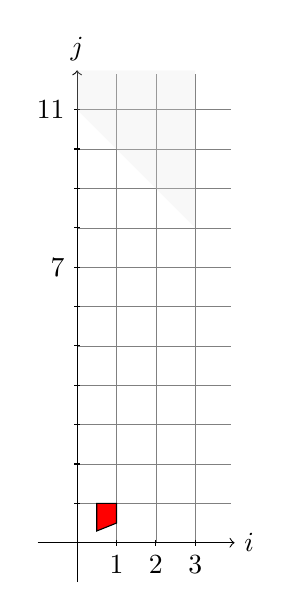
\begin{tikzpicture}[scale=0.5]

\draw (1.05cm,2pt) node[above]{};
 %  {$\displaystyle\int_0^{3/2} \!\!x^2\mathrm{d}x$};

\draw[style=help lines] (0,0) grid (3.9,11.9);
  % [step=0.25cm]      (1,2) grid +(1,1);

\draw[->] (-1,0) -- (4,0) node[right] {$i$};
\draw[->] (0,-1) -- (0,12) node[above] {$j$};

\foreach \x/\xtext in {1/1, 2/2, 3/3}
\draw[shift={(\x,0)}] (0pt,2pt) -- (0pt,-2pt) node[below] {$\xtext$};

\foreach \y/\ytext in {1/, 2/, 3/,4/,5/,6/,7/7,8/, 9/, 10/, 11/11}
\draw[shift={(0,\y)}] (2pt,0pt) -- (-2pt,0pt) node[left] {$\ytext$};

\draw[fill=red]  (0.5,0.3) -- (0.5,1) -- (1,1) -- (1,0.5) -- cycle;
\fill[gray!20,nearly transparent] (0,11) -- (0,12) -- (3,12) -- (3,8) -- cycle;
% \fill[gray!20] (0,11) -- (0,12) -- (3,12) -- (3,8) -- cycle; %without transparency
\end{tikzpicture}

\printbibliography{}
\end{document}
